\documentclass{article}
\usepackage{alltt,gdefs,epsfig}

%\usepackage[inactive]{srcltx} % SRC Specials for DVI Searching

% Over-full v-boxes on even pages are due to the \v{c} in author's name
\vfuzz2pt % Don't report over-full v-boxes if over-edge is small

\newcommand{\lemref}[1]{Lemma~\ref{Lm:#1}}
\newcommand{\figref}[1]{Figure~\ref{Fi:#1}}
\newcommand{\defref}[1]{Definition~\ref{De:#1}}
\newcommand{\tableref}[1]{Table~\ref{Ta:#1}}
\newcommand{\subsubsubsection}[1]{\emph{#1}:}
\newcommand{\impliesT}{\ \makebox{$\triangleright$}\ }
\newcommand{\threeValue}[3]{{\lsyn #1 \rsyn_3^{#2}(#3)}}
\newcommand{\evaluate}[3]{{\lsyn #1 \rsyn^{#2}(#3)}}
\newcommand{\twoValue}[3]{\lsyn{#1}\rsyn_2^{#2}(#3)}
\newcommand{\lt}{$<$}
\newcommand{\gt}{$>$}
\newcommand{\deref}{\makebox{{\tt ->}}}
\newcommand{\PVar}{{\it PVar}}
\newcommand{\param}[1]{$<$#1$>$}
\newcommand{\freeVars}{{\it freeVars\/}}
\newcommand{\closure}{{\it closure\/}}
\newcommand{\blur}{{\it blur\/}}
\newcommand{\coerce}{{\it Coerce\/}}
\newcommand{\foreach}{\textbf{foreach}}
\newcommand{\predbox}{\textbf{box}}
\newcommand{\foreachI}{\textbf{for}\=\+\textbf{each}}
\newcommand{\unique}{\textbf{unique}}
\newcommand{\function}{\textbf{function}}
\newcommand{\invfunction}{\textbf{invfunction}}
\newcommand{\symmetric}{\textbf{symmetric}}
\newcommand{\antisymmetric}{\textbf{antisymmetric}}
\newcommand{\reflexive}{\textbf{reflexive}}
\newcommand{\antireflexive}{\textbf{antireflexive}}
\newcommand{\transitive}{\textbf{transitive}}
\newcommand{\tvtitle}{\textbf{\%t}}
\newcommand{\seperator}{\textbf{\%\%}}
\newcommand{\tvimpl}{\deref}
\newcommand{\STRUCT}[1]{\mbox{3-STRUCT}[#1]}
\newcommand{\Voc}{{\cal P}}

\newcommand{\CRewrites}{\C{\Rightarrow}}
\newcommand{\Rewrites}{\Rightarrow}
\newcommand{\heldby}{held\_by}
\newcommand{\isacquired}{is\_acquired}
\newcommand{\propertyoccurred}{property\_occurred}
\newcommand{\isblocked}{is\_blocked}
\newcommand{\iswaiting}{is\_waiting}
\newcommand{\rby}{r\_by}
\newcommand{\isthread}{isthread}
\newcommand{\ready}{ready}
\newcommand{\waitfor}{wait\_for}
\newcommand{\tvmc}{$3$VMC}
\newcommand{\new}{\textbf{\%new}}
\newcommand{\newthread}{\textbf{\%newthread}}
\newcommand{\retain}{\textbf{\%retain}}
\newcommand{\tstart}{\textbf{\%start}}
\newcommand{\tstop}{\textbf{\%stop}}
\newcommand{\tvhalt}{\textbf{\%halt}}
\newcommand{\tvfocus}{\textbf{\%f}}
\newcommand{\tvprecond}{\textbf{\%p}}
\newcommand{\tvmessage}{\textbf{\%message}}
\newcommand{\tvinclude}{\textbf{\%include}}
\newcommand{\tvexclude}{\textbf{\%exclude}}
\newcommand{\tvexplicitat}{\textbf{\%explicitat}}

\setcounter{topnumber}{5}
\def\topfraction{0.99}
\def\textfraction{0.05}
\def\floatpagefraction{0.9}
\setcounter{bottomnumber}{5}
\def\bottomfraction{0.99}
\setcounter{totalnumber}{10}
\def\dbltopfraction{0.99}
\def\dblfloatpagefraction{0.8}
\setcounter{dbltopnumber}{5}

%\author{Eran Yahav \thanks{Computer Sciences Department, School of
%Mathematical Science, Tel-Aviv University, Tel-Aviv 69978, Tel:
%+972-3-6407606, Fax: +972-3-6406761, yahave@math.tau.ac.il.}} \and
%Mooly Sagiv \thanks{Computer Sciences Department, School of
%Mathematical Science, Tel-Aviv University, Tel-Aviv 69978, Tel:
%+972-3-6407606, Fax: +972-3-6406761, sagiv@math.tau.ac.il.}

\author{Eran Yahav\thanks{School of Computer Science, Tel-Aviv University, Tel-Aviv 69978, Israel
Tel: +972-3-6407606, Fax: +972-3-6406761 ; yahave@math.tau.ac.il}}

%%% ----------------------------------------------------------------------
\begin{document}


\nocite{kn:SRW99} \nocite{CGP99}


\title {$3$VMC User's Manual \\
        \smallskip
        \large{draft version} }

%%\email{yahave@math.tau.ac.il}

\date{January 27, 2001}

%%% ----------------------------------------------------------------------

\maketitle

\begin{abstract}
$3$VMC is a model checker which uses abstraction based on
$3$-valued logic. $\tvmc$ is an extension of the TVLA framework.
This document is a user's manual for $\tvmc$.
\end{abstract}

%%% ----------------------------------------------------------------------
\maketitle
%%% ----------------------------------------------------------------------


\section{Introduction}

$\tvmc$ is a tool for analysis and verification of concurrent
systems. In contrast to existing verification tools (e.g.
\cite{lncs962*453}) $\tvmc$ is geared towards verification of
concurrent software with dynamic allocation of objects and
threads. $\tvmc$ provides a powerful abstraction mechanism by
using $3$-valued logic to represent multiple program
configurations. $\tvmc$ is an extension of the TVLA framework
\cite{kn:TalSAS00}. Theoretical background for $\tvmc$ can be
found in \cite{Yahav01}.

\begin{figure}
\begin{center}
\framebox{ \vbox{
\begin{alltt}
\begin{tabbing}

pu\=blic class Client implements Runnable \{ \+ \\
    pu\=blic void run() \{ \+ \\
      wh\=ile (true) \{ \+ \\
        sy\=nchronized(lock) \{ \+ \\
            // do some critical stuff \- \\
        \} \- \\
      \} \- \\
    \} \- \\
\} \\

pu\=blic class Main \{ \+ \\
  pu\=blic static void main() \{ \+ \\
    Thread t1 = new Thread(new Client()); \\
    Thread t2 = new Thread(new Client()); \\
    Thread t3 = new Thread(new Client()); \\
    t1.start(); \\
    t2.start(); \\
    t3.start(); \- \\
  \} \- \\\
\} \\

\end{tabbing}
\end{alltt}
} }
\end{center}
\caption{\label{Fi:MutexJava}Mutual exclusion example program.}
\end{figure}


In this paper, we will show how to perform verification of the
simple Java program given in \figref{MutexJava}.

\section{Three-Valued Configurations}

A \emph{program configuration} encodes a global state of a program
which consists of (i)~a global store, (ii)~the program-location of
every thread, and (iii)~the status of locks and threads, e.g., if
a thread is waiting for a lock. Technically, we use first-order
logic with transitive-closure to express configurations and their
properties in a parametric way. Formally, we assume that there is
a set of predicate symbols $P$ for every analyzed program each
with a fixed arity. For example, \tableref{Predicates} contains
predicates for partial semantics of Java. The predicates above the
double-line separator are internal $\tvmc$ predicates. The
predicates below the separator are defined by the user who wishes
to capture the thread-semantics of Java.

\begin{itemize}
\item The unary predicate $\isthread(t)$ is used to denote the
objects that are threads. (e.g., in Java - instances of a subclass
of \texttt{class Thread}).
\item For every potential program-location (program label) $lab$ of
a thread $t$, there is a unary predicate $at[lab](t)$ which is
true when $t$ is at $lab$. These predicates will be referred to as
\emph{location predicates}.
\item For every class field and function
parameter \texttt{fld}, a binary predicate $rvalue[fld](o_1,o_2)$
records the fact that the \texttt{fld} of the object $o_1$
pointing to the object $o_2$.
\item The predicates $held\_by(l,t)$, $blocked(t,l)$ and $waiting(t,l)$
model possible relationships between locks and threads.
%\item The predicate $held\_by(l,t)$ is true when the lock $l$
%is acquired by the thread $t$, via a successful
%\texttt{synchronized} statement.
%\item The predicate $blocked(t,l)$ is true when the thread $t$ is
%blocked on the lock $l$, as a result of an unsuccessful
% \texttt{synchronized} statement.
%\item The predicate $waiting(t,l)$ is true when the thread $t$
%is waiting for the lock $l$ as a result of invoking a
%\texttt{wait()} call.
%\item The predicate $idlt(l_1,l_2)$ is used to record a
%partial order between objects. Each object is assumed to have a
%unique id. The predicate $idlt(l_1,l_2)$ is true when the id of
%$l_1$ is less than the id of $l_2$. The order between objects can
%be used for deadlock prevention by breaking cyclic allocation
%requests \cite{IB-D943023}. In Section~\ref{Se:ResourceOrdering}
%we show how our technique can be used to verify that a program
%uses such a resource-allocation policy.
\end{itemize}


Configurations are depicted as directed graphs. Each individual
from the universe is displayed as a node. A unary predicate $p$
which holds for an individual (node) $u$ is drawn inside the node
$u$. The name of a node is written inside angle brackets. Node
names are only used for ease of presentation and do not affect the
analysis. A true binary predicate $p(u_1,u_2)$ is drawn as
directed edge from $u_1$ to $u_2$ labeled with the predicate
symbol. \figref{Concrete} shows a configuration which consists of
4 threads competing for an exclusive shared resource.

\begin{figure*}
\begin{center}
\framebox{
    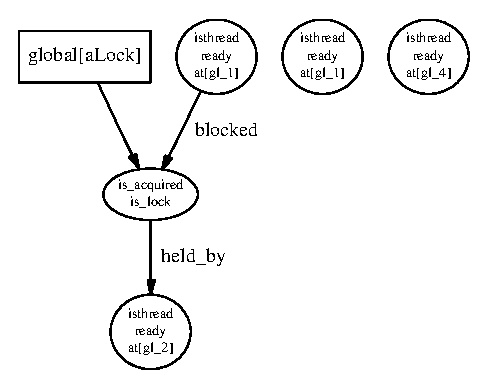
\epsfig{file=figures/concrete,width=3in} %width=4.8in
}
\end{center}
\caption{\label{Fi:Concrete}A concrete configuration
$\C{C_{\ref{Fi:Concrete}}}$.}
\end{figure*}




\begin{table}
\begin{center}
\begin{tabular}{|l|l|} \hline
  % after \\ : \hline or \cline{col1-col2} \cline{col3-col4} ...
  \textbf{Predicates} & \textbf{Intended Meaning} \\
  \hline \hline
  $\isthread(t)$ & \begin{tabular}{l} $t$ is a thread \end{tabular}\\
  \hline
  $\ready(t)$ & \begin{tabular}{l} $t$ is ready for scheduling \end{tabular}\\
  \hline
  $\begin{array}{l}
  \{ at[lab](t) : \\
  ~~~lab \in Labels \}
  \end{array}$ & \begin{tabular}{l} thread $t$ is at label $lab$ \end{tabular} \\
  \hline
  \hline
  $\begin{array}{l}
  \{ rvalue[fld](o_1,o_2) : \\
  ~~~fld \in Fields \}
  \end{array}$ &
  \begin{tabular}{l}
    field $fld$ of the object $o_1$ \\
    points to the object $o_2$ \\
  \end{tabular} \\
  \hline
  $held\_by(l,t)$ & \begin{tabular}{l} the lock $l$ is held by \\ the thread $t$\\
  \end{tabular} \\
  \hline
  $blocked(t,l)$ & \begin{tabular}{l} the thread $t$ is blocked \\ on the lock $l$\\
  \end{tabular} \\
  \hline
  $waiting(t,l)$ &
  \begin{tabular}{l} the thread $t$ is waiting \\ on the lock $l$\\
  \end{tabular} \\
  \hline
  %$idlt(l_1,l_2)$ &
%  \begin{tabular}{l}
%  the id of lock $l_1$ is \\
%  less than the id of lock $l_2$ \\
%  \end{tabular} \\
%  \hline
  %%$runnable(t)$ & is thread $t$ scheduled to execute ? \\
  %%\hline
\end{tabular}
\end{center}
\caption{\label{Ta:Predicates}Predicates for partial Java
semantics.}
\end{table}

$\tvmc$ conservatively represent multiple configurations using a
single logical structure but with an extra truth-value $1/2$
denoting values which may be $1$ and may be $0$. The values $0$
and $1$ are called \emph{definite values} where the value $1/2$
is called \emph{indefinite value}.

\section{Three-Valued Models}

A three-valued model defines the behavior of the program to be
verified. It defines the effect of \emph{actions} and how actions
are applied to configurations. A three-valued model consists of
the following:
\begin{itemize}
\item Declarations
\item Action Definitions
\item Thread Types Definitions
\item Properties
\item Output Modifiers
\end{itemize}

\begin{figure}
\begin{center}
\framebox{ \vbox{
\begin{alltt}
\begin{tabbing}

/*** \\
** mutex.tvm \\
** mutual exclusion examples for unbound number of threads. \\
** based on the example from "symmetry and model checking" \\
***/ \\


/*********************** Sets ******************************/ \\
\%s FieldsAndParameters \{ \} \\
\%s Globals \{ aLock \} \\

/**************** Predicates **************/ \\

\#include "con\_pred.tvm" \\
\#include "shape\_pred.tvm" \\

\%p \propertyoccurred() \\

\seperator \\
/********************* Actions *******************/ \\

\#include "con\_stat.tvm" \\

\%action verifyProperty() \{ \\
    \tvprecond  !\propertyoccurred() \\
    \tvmessage\= (E(t\_1,t\_2) (t\_1 != t\_2) \& at[gl\_2](t\_1) \& at[gl\_2](t\_2)) \+ \\
    ->  "mutual exclusion may be violated" \- \\
\} \\

/**************** Program *********************/ \\

\seperator \\

/***********************************************/ \\
/**************  Threads ****************/ \\

\%thread \= main \{ \+ \\                     \=
        $gl_1$ blockLockGlobal(aLock) $gl_1$        \` // lock(aLock) \\
        $gl_1$ succLockGlobal(aLock) $gl_2$         \`              \\
        $gl_2$ skip() $gl_3$                        \`              \\
        $gl_3$ unlockGlobal(aLock) $gl_4$           \` // unlock(aLock) \- \\
\} \\

\seperator \\
/**********************************************/ \\
/************** Claims        ****************/ \\
verifyProperty() \\

\end{tabbing}
\end{alltt}
} }
\end{center}
\caption{\label{Fi:TmutexTVM}TVM file for mutual exclusion
example.}
\end{figure}


\figref{TmutexTVM} shows the TVM file for the mutual exclusion
example program.

\subsection{Declarations}

The declarations section of a three-valued model may consist of
declarations of \emph{core predicates}, \emph{intrumentation
predicates}, sets and consistency rules. The reader is referred to
\cite{kn:TalSAS00} for more details.

$\tvmc$ automatically defines the predicates above the two-line
separator of \tableref{Predicates}. In addition, $\tvmc$ defines
the set $Labels$ which contains all labels in the program.


\subsection{Action Definitions}

Informally, an action is characterized by the following kinds of
information:
\begin{itemize}
\item A {\em precondition\/} under which the action is \emph{enabled} expressed
as logical formula. This formula may also include a designated
free variable $t_r$ to denote the ``scheduled'' thread on which
the action is performed. Our operational semantics is
non-deterministic in the sense that many actions can be enabled
simultaneously and one of them is chosen for execution. In
particular, it selects the scheduled thread by an assignment to
$t_r$.

\item An \emph{enabled} action creates a new configuration where the
interpretations of every predicate $p$ of arity $k$ is determined
by evaluating a formula $\varphi_p(v_1, \ldots, v_k)$ which may
use $v_1, \ldots, v_k$ and $t_r$ as well as all other predicates
in $P$.
\end{itemize}

A program statement may be modeled by several alternative actions
corresponding to the different behaviors of the statement. A
single action to be taken is determined by evaluation of the
preconditions.

Technically, an action consists of the following:
\begin{itemize}
\item Title - ($\tvtitle$) a textual title for the action.
\item Focus formulae ($\tvfocus$) - focus formulae for the action, applied
before the precondition is evaluated.
\item Precondition formula ($\tvprecond$) - evaluated to determine if the action
is \emph{enabled} (could be applied) for a given configuration.
The precondition formula may have free variables, in which case,
the action is applied for every assignment that may satisfy the
formula. A special free variable $t_r$ denotes the ``scheduled''
thread on which the action is performed.
\item Universe modifiers ($\new$, $\newthread$, $\retain$) - universe modifiers allow to add/remove
individuals and thread-individuals to the universe of the
configuration.
\item Thread state modifiers ($\tstart$, $\tstop$)- allow to start and stop a thread.
An unary formula must be supplied to identify threads to be
affected by the modifier.
\item Analysis Control ($\tvhalt$) - halts the analysis.
\item Update formulae - update the configuration to model the
effect of the action.
\end{itemize}



\subsection{Thread Types}

$\tvmc$ allows the user to define thread-types. A thread-type is
defined using the keyword \texttt{\%thread} followed by the
thread-type name and the control-flow for the thread-type. A
thread-type can be later instantiated as explained in the
following section.

\figref{ThreadDef} shows a definition of a thread-type named
\emph{main} which consists of 4 actions.

\begin{figure}
\begin{center}
\framebox{ \vbox{
\begin{alltt}
\begin{tabbing}

\%thread \= main \{ \+ \\                     \=
        $gl_1$ blockLockGlobal(aLock) $gl_1$        \` // lock(aLock) \\
        $gl_1$ succLockGlobal(aLock) $gl_2$         \`              \\
        $gl_2$ skip() $gl_3$                        \`              \\
        $gl_3$ unlockGlobal(aLock) $gl_4$           \` // unlock(aLock) \- \\
\} \\

\end{tabbing}
\end{alltt}
} }
\end{center}
\caption{\label{Fi:ThreadDef}Definition of a thread type.}
\end{figure}


\subsubsection{Thread Control-flow}

Control flow in a thread-type is expressed in terms of
transitions. A transition consists of a source-label, an action,
and a target-label. CFG nodes are implicitly defined for each
label when a transition using these labels is defined. $\tvmc$
supports non-determinism when more than one enabled transition
exists from a single CFG node.

$\tvmc$ assumes that threads are scheduled arbitrarily, and thus
thread actions may be arbitrarily interleaved with actions of
other threads. A special keyword \textbf{atomic} may be used to
define atomic blocks as explained in Section~\ref{Se:Atomic}.

The values of the predicates $at[lab](tr)$ are automatically
updated when an action is applied to express the change of
$at[lab](tr)$ according to the transition. It is possible to
disable automatic update of $at[lab](tr)$ predicates by using the
keyword \tvexplicitat in the action definition header. When
explicit update is enable (automatic update disabled), the user
should provide predicate-update formulae for $at[lab](tr)$ as part
of the action's update formulae.

\subsubsection{Instantiation of Threads}

A new thread can be instantiated using the universe-modifier
$\newthread$. The universe modifier $\newthread$ takes a name of a
thread-type as parameter and create a new thread individual of the
given type. The predicate $isNew(v)$ evaluates to true for the
newly created thread node. The predicate $isNew(v)$ can be used by
the action's update formulae. A created thread is initially not
ready for scheduling.

\subsubsection{Thread Scheduling}

The thread-state modifiers $\tstart$ and $\tstop$ allow to add
thread control in an action. The modifiers require an unary
formula to identify threads to be affected by the modifier. The
unary predicate $ready(v)$ evaluates to $true$ for thread
individuals that are ready for scheduling.

\subsubsection{Analysis Control}

The $\tvhalt$ modifier allows an action to be used to halt the
analysis. When an action with the $\tvhalt$ modifier is applied,
the analysis terminates \emph{immediately}.


\subsection{Atomic Blocks}\label{Se:Atomic}

The keyword \textbf{atomic} is used to define a sequence of
actions that should be performed atomically. An atomic block is
defined using the atomic keyword followed by the block in curly
braces. An atomic block should have a single exit.

\subsection{Assertions}

The keywords \textbf{\%assert} and \textbf{hardassert} can be used
to define assertion statements. If the formula $f$ supplied to
\textbf{\%assert(f)} evaluates to \emph{true} or \emph{unknown},
the statement has no effect. If the formula evaluates to
\emph{false}, the statement will yield an error. The
\textbf{\%hardassert(f)} statement is similar to
\textbf{\%assert(f)}, but yields an error when $f$ evaluates to
\emph{unknown} in addition to \emph{false}.

Note that assertion statements simply save the need for
declaration of \emph{halting actions}.


\subsection{Properties}

Properties are implemented more generally as \emph{global
actions}. Global actions are evaluated on every step of the
analysis regardless of current active threads, current location
and current thread scheduling. A global action may perform any
required action, but it is common to use it only for evaluating a
required property.

\subsection{Output Modifiers}

The output modifiers section allows the user to define which
configurations are written to the output file. The keywords
$\tvinclude$ and $\tvexclude$ are used to define configurations
that should be included in the output or excluded from it.
$\tvinclude$ and $\tvexclude$ take a closed formula as a
parameter. Only configurations for which the formula may evaluate
to \emph{true} are included/excluded. (NYI)

\section{Initial Configurations}

A new set of nodes denoted by \%t corresponds to the threads in
the initial configuration. For example: \%t = \{ $s_t(main)$ \}
defines a new thread instance of thread-type "main". The name of
the instance is $``s_t''$. Unless explicitly stated by the
$ready(v)$ predicate, the thread is assumed to be not ready for
scheduling. The thread starts execution from its entry label. You
may create a configuration in which a thread starts at a given
label, by supplying the initial label as a second parameter -
$s_t(main,gl_3)$.

\figref{TmutexTVS} shows an initial configuration for the mutual
exclusion example. This initial configuration consists of a
summary node of threads, and a single lock. Note that the thread
node \emph{s\_t} is given the value $1/2$ for the predicate
\textbf{sm} to denote the fact that it is a summary node.


\begin{figure}
\begin{center}
\framebox{ \vbox{
\begin{alltt}
\begin{tabbing}

\%t = \{ s\_t(main) \} \\
\%n = \{ u \} \\
\%p = \= \{ \+ \\
    sm = \{ s\_t: 1/2 \} \\
    ready = \{ s\_t \} \\
    is\_lock = \{ u \} \\
    global[aLock] = \{ u \} \- \\
\} \\

\end{tabbing}
\end{alltt}
} }
\end{center}
\caption{\label{Fi:TmutexTVS}TVS file for mutual exclusion
example.}
\end{figure}


\section{Property Verification}

\subsection{Safety Properties}

Verification of safety properties is performed by exploring the
state-space, identifying configurations that may violate the
property requirements.

\figref{Explore} shows a depth-first search algorithm for
exploring a state-space. For each configuration $C$ such that $C$
is not already a \emph{memeber} of the \emph{state-space}, we
explore every configuration $C'$ that can be produced by applying
some action to the current configuration $C$. Note that the
$verify$ step checks if the current configuration $C$ satisfies
the property requirements.

\begin{figure}
\begin{center}
\framebox{ \vbox{
\begin{alltt}
\begin{tabbing}

init\=ialize($C_{0}$) \{ \+ \\
    for \=each $C \in C_{0}$ \+ \\
        push(stack,C) \- \- \\
\} \\


ex\=plore() \{ \+ \\
  wh\=ile stack is not empty \{ \+ \\
    $C$ = pop(stack) \\
    \emph{verify(C)}     \\
    if \= not $member(C,stateSpace)$ \{ \+ \\
      $stateSpace' = stateSpace \cup \{ C \} $ \\
      fo\=r each action $ac$ \+ \\
        fo\=r each $C'$ such that $ C \Rewrites_{ac} C'$  \+ \\
            push(stack,$C'$) \- \- \- \\
    \} \- \\
  \} \- \\
\}

\end{tabbing}
\end{alltt}
} }
\end{center}
\caption{\label{Fi:Explore}State space exploration.}
\end{figure}


The $verify$ step actually executes all \emph{global actions}
defined by the user. The \emph{global actions} can be used issue
messages or to halt analysis when a property is violated.

\subsection{LTL Properties}

$\tvmc$ supports verification of general LTL properties by using
Buchi automata to represent the (negation of the) property to be
verified.

$\tvmc$ takes as input a \texttt{BUC} file that models the Buchi
automaton for the negation of the property to be verified.
Currently, $\tvmc$ does not support automatic construction of the
Buchi automaton from an LTL formula. The Buchi automaton should be
supplied by the user using the \texttt{BUC} file.

A \texttt{BUC} file consists of two parts - the first section of
the file defines the instrumentation predicates to be used as the
vocabulary of the automaton, the second section defines automaton
states and transitions (and the initial state). The sections are
separated by a special separator (\%\%).

Vocabulary instrumentation predicates are nullary predicates
defined in the same manner as in the TVM file.

Automaton is described using transition as seen in
\figref{bucFile}.

\begin{figure}
\begin{center}
\framebox{ \vbox{
\begin{alltt}
\begin{tabbing}

\%i i\_1() = E(v) isthread(v) \\
\%i i\_2() = E(v) E(l) isthread(v) \& blocked(v,l) \\
\%\% \\
\%b\=uchi example \{ \+ \\
    ->(b1) \\
    (b1) i\_1 b2 \\
    b2 i\_2 b3 \\
    b3 i\_1 b4 \\
    b4 i\_2 b5 \\
    b5 i\_1 (b1) \- \\
    \} \\
\end{tabbing}
\end{alltt}
} }
\end{center}
\caption{\label{Fi:bucFile}BUC file defining a Buchi automata.}
\end{figure}


Accepting states of the Buchi automaton are written as $(s)$, an
accepting state should always appear inside parentheses. The
initial state of the automaton should be defined in the first line
of automaton description using $\rightarrow$. Other transitions
are defined by triples of state-label-state, where the label
corresponds to one of the vocabulary predicates.

\input{summary}

\appendix
\section{On-line Resources}

$\tvmc$ uses the \emph{GraphViz} package to display results.
GraphViz can be obtained at:
http://www.research.att.com/sw/tools/graphviz/download.html

Additional examples and updated version of $\tvmc$ can be
downloaded from the author's home-page at:
http://www.cs.tau.ac.il/~yahave



% ------------------------------------------------------------------------

\subsection*{Acknowledgment}
Thanks to Nurit Dor, Tal Lev-Ami, Noam Rinetskey and Alex
Warshovski.

% ------------------------------------------------------------------------

\begin{figure}
\begin{center}
\framebox{ \vbox{
\begin{alltt}
\begin{tabbing}
%\begin{verbatim}
% /***********************************************************
%* con_stat.tvm
%* include file for simple concurrency
%***********************************************************/
%\end{verbatim}

\%ac\=tion skip() \{ \+ \\
   \tvtitle "skip ()" \\
   \tvprecond !\propertyoccurred() \- \\
\} \\

\%ac\=tion succLockGlobal(glb) \{ \+ \\
    \tvtitle "SuccesfulLocGlobal (" + glb + ")" \\
    \tvfocus  \{ \isacquired(l), global[glb](l) \} \\
    \tvprecond  !\propertyoccurred() \& global[glb](l) \& (!\isacquired(l) | \heldby(l,
    tr)) \\
    \{ \\

       \heldby\=(l\_1, t\_1) = \+ \\
            (\heldby(l\_1, t\_1) \&  (t\_1 != tr | l\_1 != l)) | \\
            (t\_1 == tr \& l\_1 == l) \- \\
       blocked(t\_1,l\_1) = blocked(t\_1,l\_1) \& ((t\_1 != tr) | (l\_1 != l)) \\
       \isacquired(l\_1) = \isacquired(l\_1) | (l\_1 == l) \\
   \} \- \\
\} \\

\%ac\=tion blockLockGlobal(glb) \{ \+ \\
    \tvtitle "blockLocGlobal (" + glb + ")" \\
    \tvfocus \{ global[glb](l) \& \isacquired(l) \} \\
    \tvprecond  !\propertyoccurred() \& global[glb](l) \& \isacquired(l) \&
    !\heldby(l,tr) \\
    \{ \\
        blocked\=(t\_1, l\_1) = \+ \\
            (blocked(t\_1, l\_1) \&  (t\_1 != tr | l\_1 != l)) | \\
            (t\_1 == tr \& l\_1 == l) \- \\
   \} \- \\
\} \\

\%ac\=tion unlockGlobal(glb) \{ \+ \\
    \tvtitle "unLocGlobal (" + glb + ")" \\
    \tvfocus \{ \isacquired(l), global[glb](l) \} \\
    \tvprecond !\propertyoccurred() \& global[glb](l) \\
    \{ \\
        \heldby(l\_1, t\_1) = \heldby(l\_1, t\_1) \&  (t\_1 != tr | l\_1 != l) \\
        \isacquired(l\_1) = \isacquired(l\_1) \& (l\_1 != l) \\
   \} \- \\
\} \\

\end{tabbing}
\end{alltt}
} }
\end{center}
\caption{\label{Fi:ConcTVM}TVM file for simple concurrency
semantics.}
\end{figure}


%GATHER{Xbib.bib}   % For Gather Purpose Only
%GATHER{Paper.bbl}  % For Gather Purpose Only
\bibliographystyle{amsplain}
\bibliography{c:/papers/bib/concurrent,c:/papers/bib/df,c:/papers/bib/modelcheck}
\end{document}
% ------------------------------------------------------------------------
